\documentclass[11pt,table]{article}
\usepackage[legalpaper, portrait, margin=2cm]{geometry}
\usepackage{fancyhdr}
\usepackage{biblatex}
\addbibresource{bibliography/bibliography.bib}
\usepackage{float}
\usepackage{vhistory}
\usepackage{graphicx}
\usepackage{pdfpages}
\graphicspath{{image/}}
\usepackage{amsmath}
\usepackage[hidelinks]{hyperref}
\usepackage{listings}
\usepackage{parskip}
\usepackage{xcolor}
\usepackage{lscape}
\usepackage{geometry}
\usepackage{tabularx}
\usepackage{svg}
\newcolumntype{L}{>{\raggedright\arraybackslash}X}
\usepackage{multicol}
\usepackage{setspace}
\linespread{1.3} %One and a half line height (1.6 is double line height)
\usepackage{wrapfig}
\usepackage{pdfpages}
\usepackage{subcaption}

\usepackage{subfiles} % Always Load last

\definecolor{codegreen}{rgb}{0,0.6,0}
\definecolor{codegray}{rgb}{0.5,0.5,0.5}
\definecolor{codepurple}{rgb}{0.58,0,0.82}
\definecolor{backcolour}{rgb}{0.95,0.95,0.92}

\lstdefinestyle{code_style}{
    backgroundcolor=\color{backcolour},   
    commentstyle=\color{codegreen},
    keywordstyle=\color{magenta},
    numberstyle=\tiny\color{codegray},
    stringstyle=\color{codepurple},
    basicstyle=\ttfamily\footnotesize,
    breakatwhitespace=false,         
    breaklines=true,                 
    captionpos=b,                    
    keepspaces=true,                 
    numbers=left,                    
    numbersep=5pt,                  
    showspaces=false,                
    showstringspaces=false,
    showtabs=false,                  
    tabsize=2
}

\lstset{style=code_style}

\hypersetup{colorlinks=true, linkcolor=black, urlcolor=blue, filecolor=magenta, urlcolor=cyan}
\urlstyle{same}


\title{SPRO3 report}
\date{08/09/2023}
\author{Botond Bencsik\\Casper Hvide Bjerre Simenel\\Felix Leo Hoch\\Henrik Maarten Bongers\\Laura Barney\\Arthur Kibalama}

\pagestyle{fancy}
\fancyhead[L]{\leftmark}
\fancyhead[R]{\rightmark}
\setlength{\headheight}{13.59999pt}
\addtolength{\topmargin}{-1.59999pt}


\begin{document}
\maketitle
\begin{figure}[H]
    
\includegraphics[width=\textwidth]{forklift_m.jpg}
\end{figure}
\newpage
\tableofcontents
\newpage
\section{Introduction}
    \subfile{Introduction/introduction.tex}  
\section{Problem Formulation}
    \subfile{Problem Formulation/idontknowifthisisonlyproblemformulation.tex}
    \subfile{Consideration/similar_products.tex}
    \subfile{Problem Formulation/requirement_list_1.tex}

    \subfile{Consideration/technical_considerations.tex}
    \subfile{Problem Formulation/interview.tex}
\section{Management}
    In response to the challenges outlined in the problem formulation, our approach
    to project management gained significant importance. Delving into the details
    of the requirements, we engaged in comprehensive discussions to formulate a
    robust plan. This section provides a detailed exploration of the methodologies
    employed to effectively manage project timelines, ensuring a strategic and
    well-coordinated effort towards successful project completion.
    \subfile{Management/managment.tex}
    \subfile{Management/stage_division.tex}
\section{Consideration}
    To give a good overview over what option there a available for obtaining
    specified functionalities, a mind map was created.
    \begin{figure}[H]
        \centering
        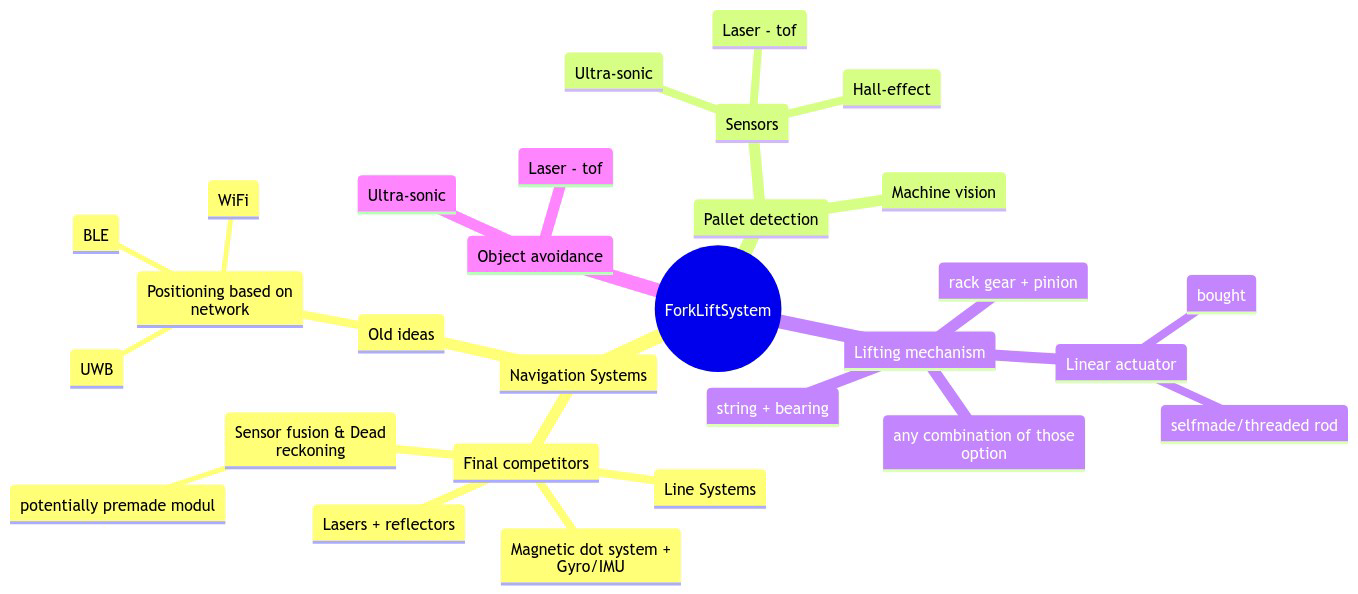
\includegraphics[width=0.8\linewidth]{MindmapForkliftSystemSolutions.md.1.png}
        \caption{Options to consider}
    \end{figure}   
    The mind map gave a good inside what topics to research further into before
    making any final chooses.
    \subfile{Consideration/forklift_functionalities.tex}
    \subfile{Consideration/lift_solutioons.tex}
    \subfile{Consideration/micro_controller.tex}
    \subfile{Consideration/morphology.tex}
\section{Electronics}
    \subfile{Electronics/ElectronicsIntro.tex}
    \subfile{Electronics/Research weight sensor.tex}
    \subfile{Electronics/ElectronicsWeightsensorInterface.tex}
   % \subfile{Electronics/Research weight sensor.tex}
   % \subfile{Electronics/ElectronicsPowersupply.tex}
   % \subfile{Electronics/ElectronicsMotordriver.tex}
\section{Mechanical}
    \subfile{Mechanical/Manufacturing.tex}
    \subfile{Mechanical/SPRO3-PartNumbering.tex}
    \subfile{Mechanical/Versions.tex}
    \subfile{Mechanical/Assembly.tex}
    \subfile{Mechanical/Lifting_development.tex}
    
\section{Code}
    \subfile{Code/code_rtos.tex}
    \subfile{Code/code_planning.tex}
    \subfile{Code/code_adc.tex}
    \subfile{Code/code_pwm.tex}
\section{Testing}
    In the dynamic landscape of project development, the validation of system
    functionalities stands as a critical phase, ensuring that each component
    operates seamlessly and meets the defined criteria. In the evaluation of system
    functionalities, a crucial aspect lies in clearly defining the anticipated
    behavior prior to the actual testing process. This foundational step serves as
    a guide, directing the systematic examination of each aspect. In this section,
    we delve into the methodologies employed during testing, underscoring the
    significance of establishing expected behavior as a fundamental precursor.
    Additionally, a comprehensive table of test cases is presented, providing a
    detailed overview of our testing approach and outcomes.
    \subfile{Testing/how_test.tex}
    \subfile{Testing/testcases.tex}
\section{Conclusion}

\newpage
\section{Appendix}

\begin{multicols}{2}
\subfile{glossary_of_terms.tex}
\end{multicols}


\newpage
\printbibliography

\end{document}